
\chapter{Costruzioni euclidee}

Per affrontare i \lq\lq tre problemi classici\rq\rq, si deve definire formalmente il gesto intuitivo della costruzione di una figura geometrica con il solo aiuto di una riga non graduata e di un compasso. In questo capitolo verranno proposte due definizioni equivalenti di costruzione euclidea ed alcuni esempi rilevanti.

%%%%%%%%%%%%%%%%%%%%%%%%%% SEZIONE   %%%%%%%%%%%%%%%%%%%
\section{Definizioni}

%% DEFINIZIONE di costruzione euclidea
\begin{definizione} 
Dato un piano e una distanza fissata $U$, una \begin{bfseries}costruzione euclidea\end{bfseries} è una successione $(K_{0}, K_{1},..., K_{n})$, i cui elementi possono essere punti, rette, o circonferenze nel piano dato, in modo che siano verificate le seguenti condizioni:

\begin{enumerate}

\item $K_{0}$ è un punto iniziale, in posizione arbitraria nel piano e $K_{1}$, un punto a distanza fissata $U$ da $K_{0}$, in direzione arbitraria.

\item Se $K_{i}$ per $ 2 \le i \le n$ è una retta, allora essa deve passare per due punti $K_{r}$ $K_{s}$ già appartenenti alla successione, ovvero già costruiti, quindi con $r, s < i$.

\item Se $K_{i}$ per $ 2 \le i \le n$ è una circonferenza, allora deve avere come centro un punto $K_{c}$ già appartenente alla successione, e come raggio il segmento dato dalla distanza fra due punti $K_{r}$ e $K_{s}$ già appartenenti alla successione, ovvero già costruiti, quindi con $c, r, s < i$.

\item Se $K_{i}$ per $ 2 \le i \le n$ è un punto, allora può essere definito come un punto a distanza fissata $U$ da un altro punto $K_{a}$ già appartenente alla successione in direzione arbitraria, oppure può essere definito come intersezione fra due circonferenze $K_{b}$, $K_{c}$  già costruite, fra due rette $K_{d}$, $K_{e}$ già costruite, o fra una retta e una circonferenza $K_{f}$, $K_{g}$ già costruite, quindi con $a,b,c,d,e,f,g < i$. 
\end{enumerate}
\end{definizione}

\begin{osservazione}
Per poter identificare la tipologia di ogni elemento della costruzione, senza dovere necessariamente usare il diagramma, si propone la seguente notazione per i diversi $K_{i}$ della successione: 
\begin{itemize}

\item Se $K_{i}$è uno dei due punti iniziali, allora si ha rispettivamente $K_{0} := P_{0}$ e $K_{1} := P_{1}$.

\item Se $K_{i}$ è una retta per due punti $K_{r}$ e $K_{s}$, allora $K_{i} := R_{i} (K_{r}, K_{s})$;

\item Se $K_{i}$ è una circonferenza di centro $K_{c}$ e di raggio il segmento avente per estremi i punti $K_{r}$ e $K_{s}$, allora $K_{i} := C_{i} (K_{c}; \overline{K_{r}K_{s}})$;

\item Se $K_{i}$ è un punto di intersezione fra due circonferenze $C_{a}$, $C_{b}$, oppure di due rette $R_{a}$, $R_{b}$, oppure di una retta $R_{a}$ e una circonferenza $C_{b}$, allora si ha rispettivamente $K_{i} := P_{i} (C_{a},C_{b})$, $K_{i} := P_{i} (R_{a},R_{b})$ oppure $K_{i} := P_{i} (R_{a},C_{b})$.
\end{itemize}

Nel caso in cui esista più di una intersezione fra la circonferenza e la retta o fra due circonferenze, allora nella numerazione il primo dei punti sarà quello più a destra, o se sono allineati verticalmente, quello più alto dei due.
\end{osservazione}

\noindent
La seconda definizione di costruzione euclidea proposta, si avvale della definizione di operazione fondamentale, in cui viene specificata direttamente la convenzione sulle notazioni appena introdotte:

%% DEFINIZIONE di operazione fondamentale
\begin{definizione}  
Dato un piano $\mathscr{P}$, un suo punto fissato $P_{0}$ e una distanza fissata $U$, le seguenti possibilità si definiscono \begin{bfseries}operazioni fondamentali\end{bfseries}:

\begin{enumerate}

\item Tracciare un punto $P_{i}$ nel piano a distanza $U$ da un punto $P_{j}$ già costruito in direzione arbitraria; tale punto sarà indicato con $P_{i}$.

\item Tracciare una retta $R_{i}$ nel piano per due punti $P_{r}$, $P_{s}$ già costruiti; tale retta sarà indicata con $R_{i}(P_{r},P_{s})$.

\item Tracciare una circonferenza $C_{i}$ nel piano, di centro il punto $P_{c}$, già costruito e di raggio che ha per estremi i punti $P_{r}$, $P_{s}$ già costruiti; tale circonferenza sarà indicata con $C_{i} (P_{c}; \overline{P_{r}P_{s}})$.

\item Tracciare un punto $P_{i}$ nel piano, definito o come intersezione di  due circonferenze $C_{r}$ e $P_{s}$, già costruite, o come intersezione di due rette $R_{r}$ ed $P_{s}$ già costruite, o come intersezione di una retta e di una circonferenza $R_{r}$ e $C_{s}$ già costruite. Tale punto sarà indicato rispettivamente con $P_{i}(C_{r}, C_{s})$, $P_{i}(R_{r}, R_{s})$ e $P_{i}(C_{r}, R_{s})$. Nel caso in cui ci siano due intersezioni fra le figure trattate, allora il primo per numerazione sarà il più a destra oppure se sono allineati verticalmente, il più alto. 

\end{enumerate}
\end{definizione}

%% DEFINIZIONE di costruzione euclidea da operazioni fondamentali
\begin{definizione} 
Una \begin{bfseries}costruzione euclidea\end{bfseries} è una successione di operazioni fondamentali su un piano $\mathscr{P}$ il cui primo elemento è dato dal punto inizialmente fissato $P_{0}$.
\end{definizione}


%%%%%%%%%%%%%%%%%%%%%%%%%% SEZIONE   %%%%%%%%%%%%%%%%%%%
%%%%%%%%%%%%%%%%%%%%%%%%%%%%%%%%%%%%%%%%%%%%%%%%%

\section{Esempi fondamentali}

Nei seguenti sette esempi proposti si elencano le costruzioni euclidee più importanti. Gli ultimi due in particolare saranno di fondamentale importanza nel prossimo capitolo.

%
%%%%%%%%%%%%%%%%%%%%%%%%%	ESEMPIO RETTA PERPENDICOLARE %%%%
\subsection{Retta perpendicolare ad una retta data} \label{perp}

Per costruire una retta perpendicolare ad un altra retta costruita per i punti iniziali, $P_{0}$ e $P_{1}$, si procede nel seguente modo:

\begin{enumerate}

\item Si tracci il punto $P_{1}$ a distanza $U$ da $P_{0}$ in direzione arbitraria.

\item Si tracci la retta $R_{2}(P_{0}, P_{1})$, passante quindi per i punti $P_{0}$ e $P_{1}$.

\item Si tracci la circonferenza $C_{3}(P_{0};\overline{P_{0}P_{1}})$, avente centro in $P_{0}$ e raggio di lunghezza $\overline{P_{0} P_{1}} = U$.

\item Si evidenzi il punto $P_{4}(C_{3}, R_{2} )$, intersezione fra $C_{3}$ e $R_{2}$.

\item Si tracci la circonferenza $C_{5}(P_{1};\overline{P_{1} P_{4}})$, avente centro in $P_{1}$ e raggio di lunghezza $\overline{P_{1} P_{4}} = 2U$.

\item Si tracci la circonferenza $C_{6}(P_{4};\overline{P_{1} P_{4}})$, avente centro in $P_{4}$ e raggio di lunghezza $\overline{P_{1} P_{4}} = 2U$.

\item Si evidenzi il punto  $P_{7}(C_{5}, C_{6} )$, come prima tra le due intersezioni fra $C_{5}$ e $C_{6}$.

\item Si tracci la retta $R_{8}(P_{0}, P_{7})$, passante per i punti $P_{0}$ e $P_{7}$.

\end{enumerate}

\noindent 
La retta  $R_{8}(P_{0}, P_{7})$ è perpendicolare ad $R_{2}(P_{0}, P_{1})$; 
la costruzione euclidea appena descritta è data dalla successione 


%%%%%%%% IMMAGINE COSTRUZIONE PERPENDICOLARE %
\begin{figure}[!h]
%centrare
\begin{center}
\resizebox{12.7 cm}{9.5 cm}{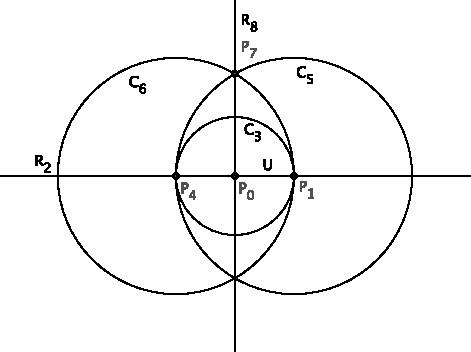
\includegraphics{1_Es1_perp}} 
%\includegraphics{Es1perpendicolare} 
\caption{Rette perpendicolari}
\end{center}
\end{figure}

%%%%%%%%%%%%%%%%%%%%%%%%%%%%%%%%%%%%%%% S1

\begin{align*}
S_{1} = ( &P_{0}, P_{1}, R_{2}(P_{0}, P_{1}), C_{3}(P_{0};\overline{P_{0} P_{1}}), \\
&P_{4}(C_{3}, R_{2} ), C_{5}(P_{1};\overline{P_{1} P_{4}}), C_{6}(P_{4};\overline{P_{1} P_{4}}),\\
&P_{7}(C_{5}, C_{6} ), R_{8}(P_{0}, P_{7}) )
\end{align*}




%%%
%%%%%%%%%%%%%%%%%%%%%%%%%% ESEMPIO ASSI CARTESIANI    %%%%%%%%%
\subsection{Sistema di assi cartesiani} \label{carte}
Per costruire un sistema di assi cartesiani, centrati in $P_{0}$ e di unità di misura $U$ data, si procede alla costruzione di due rette perpendicolari descritte dall'esempio precedente; dopodichè ciascuna retta può diventare asse del sistema cartesiano, con una ripartizione in segmenti di lunghezza $U$ attraverso la costruzione di circonferenze successive con centro nell'intersezione fra l'asse stesso e la circonferenza precedente. Si proceda nel seguente modo:

\begin{enumerate}

\item Si tracci la costruzione definita dalla successione $S_{1}$ dell'esempio precedente. 

\item Si rinominino i punti sugli assi, con una notazione più comoda: $P_{0} := P_{(0,0)}$ e $P_{1} := P_{(1,0)}$.

\item Si costruiscano le circonferenze $C_{(i,0)}(P_{(i,0)};\overline{U})$ sull'asse orizzontale di centro $P_{(i,0)}$ e di raggio $U$. Ciascuna di esse formerà due intersezioni, la prima nuova, che sarà chiamata $P_{(i+1,0)}$, e la seconda già costruita precedentemente e chiamata $P_{(i-1,0)}$, per $i = 1 ... n$

\item Si costruiscano con lo stesso procedimento del punto precedente, i punti $P_{(0,i)}$ che suddividono l'asse verticale in unità di misura di lunghezza $U$.

\end{enumerate}

\noindent
Le due rette perpendicolari $R_{2}(P_{0}, P_{1})$ e $R_{8}(P_{0}, P_{7})$ costruite formano gli assi cartesiani cercati. Le successioni di punti $P_{(i,0)}$ e $P_{(0,i)}$, suddividono gli assi nelle unità di misura del sistema.  
La costruzione euclidea appena descritta è data dalla successione:

%%%%%%%%%%%%%%%%%%%%%%%%%%%%%%%%%%%%%%% S 2

\begin{align*}
S_{2} = S_{1} \cup \{C_{(i,0)}(P_{(i,0)};\overline{U}), P_{(i+1,0)}, \mid  i \in (1,2\dots) \}  \\
 \{C_{(0,i)}(P_{(0,i)};\overline{U}), P_{(i+1,0)} \mid   i \in (1,2\dots) \} \cup \\
  \{C_{(i,0)}(P_{(i,0)};\overline{U}), P_{(i-1,0)}, \mid  i \in (-1,-2\dots) \}  \cup  \\
  \{C_{(0,i)}(P_{(0,i)};\overline{U}), P_{(i-1,0)} \mid  i \in (-1,-2\dots) \} 
\end{align*}


%%%%%%%%% IMMAGINE COSTRUZIONE ASSI % %%%%%%%%%%%%%%%%%%%%%

\begin{figure}[!h]
%centrare
\begin{center}
\resizebox{12.7 cm}{9.5 cm}{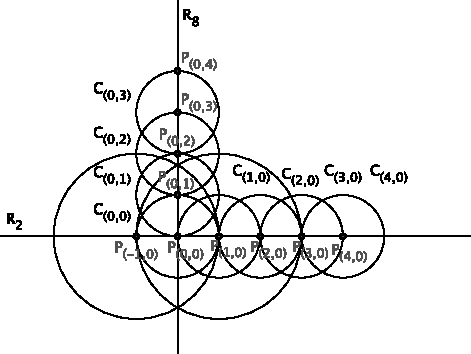
\includegraphics{1_Es_2_assi}} 
\caption{Assi cartesiani}
\end{center}
\end{figure}


%%%
%%%%%%%%%%%%%%%%%%%%%%%%%% Esempio BISETTRICE %%%%%%%%%%%%%
\subsection{Bisettrice di un quadrante} \label{bisett}
Per costruire la bisettrice dell'angolo formato fra due rette perpendicolari, si può procedere nel seguente modo:

\begin{enumerate}

\item Si tracci la successione definita dalla successione $S_{1}$ dell'esempio \ref{perp}.

\item Si evidenzi il punto $P_{9}(C_{3}, R_{8})$, come prima intersezione fra $C_{3}$ ed $R_{8}$.

\item Si tracci la circonferenza  $C_{10}(P_{9}; \overline{P_{1} P_{4}} )$.

\item Si evidenzi il punto $P_{11}(C_{5}, C_{10})$, come prima intersezione fra $C_{5}$ e $C_{10}$.

\item Si tracci infine la retta $R_{12}(P_{0}, P_{11} )$. 

\end{enumerate}

\noindent
La retta $R_{12}(P_{0}, P_{11} )$ è la bisettrice del primo e terzo quadrante cercata. La costruzione euclidea è data da:

%%%%%%%%%%%%%%%%%%%%%%%%%%%%%% S3 %%%%%%%%%%%
\begin{align*}
S_{3} = S_{1} \cup (P_{9}(C_{3}, R_{8}), C_{10}(P_{9}; \overline{P_{1}P_{4}} ),  \\
 P_{11}(C_{5}, C_{10}),  R_{12}(P_{0}, P_{11} ) ) \\
\end{align*}


%%%%%%%%% IMMAGINE COSTRUZIONE BISETTRICE ASSI %%%%%%%%%%%%%
\begin{figure}[!h]
%centrare
\begin{center}
\resizebox{12.7 cm}{9.5 cm}{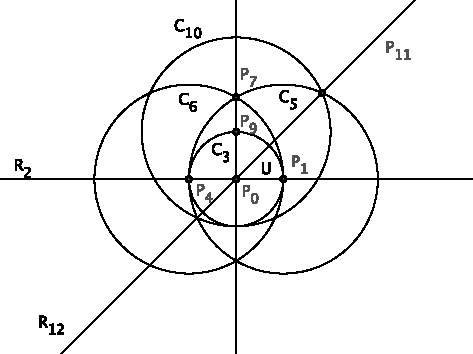
\includegraphics{1_Es3_bisett}} 
\caption{Bisettrice}
\end{center}
\end{figure}

%%%%%%%%%%%%%%%%%
%%%%%%%%%%%%%%%%%%%%%%%%%% Esempio PUNTO MEDIO%%%%%%%%%
\subsection{Punto medio} \label{medio}
Dato un segmento di estremi $P_{0}$ e $P_{1}$, procedendo nel seguente modo è possibile costruire il suo punto medio:

\begin{enumerate}

\item Si tracci il punto $P_{1}$ a distanza $U$ da $P_{0}$ in direzione arbitraria.

\item Si tracci la retta $R_{2}(P_{0}, P_{1})$.

\item Si tracci la circonferenza $C_{3}(P_{0}; \overline{P_{0} P_{1}})$.

\item Si tracci la circonferenza $C_{4}(P_{1}; \overline{P_{1} P_{0}})$.

\item Si evidenzi il primo punto di intersezione $P_{5}(C_{3},C_{4})$ fra le due circonferenze appena costruite, secondo l'ordine convenzionale.

\item Si evidenzi il secondo punto di intersezione  $P_{6}(C_{3},C_{4})$ fra le due circonferenze appena costruite, secondo l'ordine convenzionale.

\item Si tracci la retta $R_{7}(P_{5}, P_{6})$.

\item Si evidenzi il punto di intersezione $P_{8}(R_{2},R_{7})$.

\end{enumerate}

\noindent
Il punto  $P_{8}$ è il punto medio del segmento $ \overline{P_{0} P_{1}}$.
La costruzione euclidea è data da:

%%%%%%%%%%%%%%%%%%%%%%%%%%%%%% S4 %%%%%%%%%%%

\begin{align*}
S_{4} = (&P_{0}, P_{1}, R_{2}(P_{0}, P_{1}), C_{3}(P_{0}; \overline{P_{0} P_{1}}) \\
&C_{4}(P_{1}; \overline{P_{1} P_{0}}), P_{5}(C_{3},C_{4}), P_{6}(C_{4},C_{3}) \\
&R_{7}(P_{5}, P_{6}), P_{8}(R_{2},R_{7}) )
\end{align*}



%%%%%%%%% IMMAGINE COSTRUZIONE PUNTO MEDIO %%%%%%%%%%%%%

\begin{figure}[!h]
%centrare
\begin{center}
\resizebox{12.7 cm}{9.5 cm}{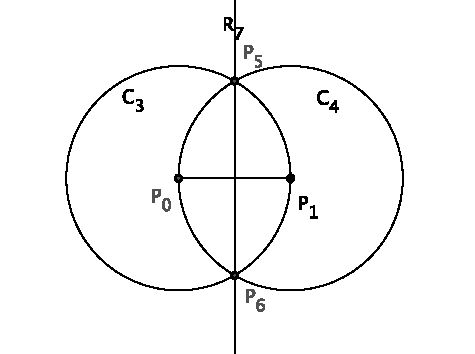
\includegraphics{1_Es4_puntomed}} 
\caption{Punto medio}
\end{center}
\end{figure} 


%%%%%%%%%
%%%%%%%%%%%%%%%%%%%%%%%%%% Esempio RETTA PARALLELA %%%%%%%%
\subsection{Retta parallela ad una retta data, per un punto dato} \label{parall}
Data una retta $R_{2}$ passante per $P_{0}$ e $P_{1}$, e un punto $P_{3}$ esterno alla retta, si richiede la costruzione con riga e compasso della parallela a $R_{2}$ passante per $P_{3}$. Per risolvere tale problema, si può applicare due volte la costruzione della perpendicolare ad una retta data, già proposto in \ref{perp}, nel seguente modo:

\begin{enumerate}

\item Si tracci il punto $P_{1}$ a distanza $U$ da $P_{0}$ in direzione arbitraria.

\item Si tracci la retta $R_{2}(P_{0}, P_{1})$, passante quindi per i punti $P_{0}$ e $P_{1}$.

\item Si evidenzi con $P_{3}$ il punto dato dal problema.

\item Si tracci la circonferenza $C_{4}(P_{3}; \overline{P_{3} P_{0}})$.

\item Si evidenzi $P_{5}(R_{2},C_{4})$, punto di intersezione fra $R_{2}$ e $C{4}$.

\item Si tracci la circonferenza $C_{6}(P_{0}; \overline{P_{0} P_{3}})$.

\item Si tracci la circonferenza $C_{7}(P_{5}; \overline{P_{5} P_{3}})$.

\item Si evidenzi $P_{8}(C_{6},C_{7})$, punto di intersezione fra $C_{6}$ e $C{7}$.

\item Si tracci la retta $R_{9}(P_{3}, P_{8})$. 

\item Si evidenzi $P_{10}(R_{2},R_{9})$, punto di intersezione fra $R_{2}$ e $R{9}$.

\item Si tracci $C_{11}(P_{3}; \overline{P_{3} P_{10}})$.

\item Si tracci il punto $P_{12}(R_{9}, C_{11})$.

\item Si tracci la circonferenza $C_{13}(P_{10}; \overline{P_{10} P_{12}})$.

\item Si tracci la circonferenza $C_{14}(P_{12}; \overline{P_{10} P_{12}})$

\item Si evidenzi $P_{15}(C_{13},C_{14})$, punto di intersezione fra $C_{13}$ e $C{14}$.

\item Si tracci la retta $R_{16}(P_{3}, P_{15})$. 

\end{enumerate}

\noindent 
La retta  $R_{16}(P_{3}, P_{15})$ è parallela alla retta data $R_{2}(P_{0}, P_{1})$ e passa per il punto dato $P_{3}$.
La costruzione euclidea appena descritta è data dalla successione: 

%%%%%%%%%%%%%%%%%%%%%%%%%%%%%%%%%%%%%%% S5

\begin{align*}
S_{5} = (&P_{0}, P_{1}, R_{2}(P_{0}, P_{1}), P_{3}, C_{4}(P_{3}; \overline{P_{3} P_{0}}) \\
&P_{5}(R_{2},C_{4}), C_{6}(P_{0}; \overline{P_{0} P_{3}}), C_{7}(P_{5}; \overline{P_{5} P_{3}}),  \\
&P_{8}(C_{6},C_{7}), R_{9}(P_{3}, P_{8}), P_{10}(R_{2},R_{9}), C_{11}(P_{3}; \overline{P_{3} P_{10}}) \\
&P_{12}(R_{9}, C_{11}), C_{13}(P_{10}; \overline{P_{10} P_{12}}) \\
&C_{14}(P_{12}; \overline{P_{10} P_{12}}), P_{15}(C_{13},C_{14}), R_{16}(P_{3}, P_{15}) )
\end{align*}

%%%%%%%% IMMAGINE COSTRUZIONE PARALLELE %
\begin{figure}[!h]
%centrare
\begin{center}
\resizebox{14.0 cm}{10.5 cm}{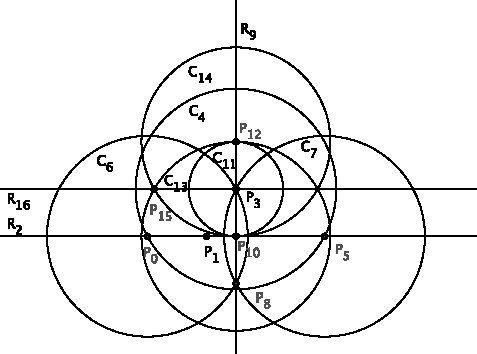
\includegraphics{1_Es5_parall}} 
%\includegraphics{Es1perpendicolare} 
\caption{Rette parallele}
\end{center}
\end{figure}


%%%
%%%%%%%%%%%%%%%%%%% ESEMPIO 2 SEGMENTI  %%%%%%%%%%%%%%%%

\subsection{Manipolazione di due segmenti}  \label{segm}

Questo particolare problema prevede, oltre all'uso di riga non graduata e di compasso, anche l'uso di due segmenti di lunghezza data. Dati quindi due segmenti $\alpha$ e $\beta$ $(\alpha > \beta)$, saranno proposte le costruzioni dei segmenti di lunghezza $\alpha + \beta$, $\alpha - \beta$, $\alpha \cdot \beta$ e $\alpha/\beta$. Inoltre verrà proposta la costruzione di $\alpha^{-1}$. Tali possibilità danno al procedimento di costruzione con riga e compasso la struttura di campo. 


%%%%%%%%%%%%%%%%%%%%%%%%%%%%%%%%%%%%%%%%%%%%%%%%%%%%%%%%%
%%% SOMMA E DIFFERENZA
\subsubsection{Somma e differenza dei segmenti dati}
Si propone il procedimento per la costruzione di $\alpha + \beta$ e $\alpha - \beta$:
\begin{enumerate}

\item Si pongano su una linea retta $R$ i segmenti dati $\alpha$ e $\beta$, in questo ordine, con un solo punto di intersezione.

\item Si evidenzi con  $P_{0}$ e  $P_{1}$ gli estremi di $\alpha$; con $P_{1}$ e $P_{2}$ gli estremi di $\beta$.

\item Si tracci la circonferenza $C_{3}(P_{1}; \overline{P_{1} P_{2}})$.

\item Si evidenzi con $P_{4}(C_{3},R)$,  l'intersezione non ancora tracciata fra la circonferenza e la retta.

\end{enumerate}

A questo punto si ha il segmento $P_{0} P_{2}$, di lunghezza $\alpha + \beta$, e il segmento $P_{0} P_{4}$ di lunghezza $\alpha - \beta$ \\ \\


%%%%%%%%% PRIMA e seconda IMMAGINE COSTRUZIONE 2 segmenti! %
\begin{figure}%
\begin{center}%
\subfigure[$\alpha + \beta$, $\alpha - \beta$]{
\resizebox{6.0 cm}{4.5 cm}{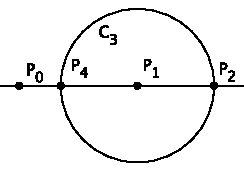
\includegraphics{1_Es6_1a}} 
}
\hspace{.20in}%
\subfigure[$\alpha \cdot \beta$]{
\resizebox{5.5 cm}{4.0 cm}{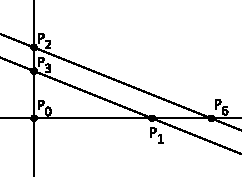
\includegraphics{1_Es6_1b}} 
}
\end{center}%
\caption{Manipolazione di segmenti 1}%
\end{figure}


%%%%%%%%%%%%%%%%%%%%%%%%%%%%%%%%%%%%%%%%%%%%%%%%%%%%%%%%%%%%% PRODOTTO
\subsubsection{Prodotto dei segmenti dati}
Si propone il procedimento per la costruzione di $\alpha \cdot \beta$:

\begin{enumerate}

\item Dopo aver costruito due rette perpendicolari centrate in $P_{0}$, si pone sull'asse orizzontale il segmento $\alpha$, con estremi $P_{0} P_{1}$ e sull'asse verticale il segmento $\beta$, con estremi $P_{0} P_{2}$.

\item Si tracci il punto $P_{3}$ a distanza $U$ da $P_{0}$, sull'asse verticale.

\item Si tracci la retta $R_{4}(P_{1}, P_{3})$.

\item Si tracci la retta $R_{5}$ parallela ad $R_{4}$ e passante per $P_{2}$, usando il procedimento dell'esempio precedente.

\item Si evidenzi il punto $P_{6}$ di intersezione fra $R_{5}$ e l'asse orizzontale. 

\end{enumerate}

Da questa costruzione, applicando il teorema di Talete, si può affermare che

\begin{align*}
\frac{P_{0}P_{6}}{\alpha} = \frac{\beta}{U}
\end{align*}

Dato che U è unità di misura iniziale, si può porre arbitrariamente uguale ad $1$, per ottenere

\begin{align*}
\frac{P_{0}P_{6}}{\alpha} = \beta
\end{align*}

Da cui si deduce che il segmento $P_{0}P_{6}$, è il segmento di lunghezza $\alpha \cdot \beta$ cercato. \\ 


%%%%%%%%%%%%%%%%%%%%%%%%%%%%%%%%%%%%%%%%%%%%%%%%%%%%%%%%%%%%% RAPPORTO
\subsubsection{Rapporto dei segmenti dati}
Si propone il procedimento per la costruzione di $\alpha/\beta$:

\begin{enumerate}

\item Dopo aver costruito due rette perpendicolari centrate in $P_{0}$, si pone sull'asse orizzontale il segmento $\alpha$, con estremi $P_{0} P_{1}$ e sull'asse verticale il segmento $\beta$, con estremi $P_{0} P_{2}$.

\item Si tracci il punto $P_{3}$ a distanza $U$ da $P_{0}$, sull'asse verticale.

\item Si tracci la retta $R_{4}(P_{1}, P_{2})$, che congiunge gli estremi di $\alpha$ e $\beta$.

\item Si tracci la retta $R_{5}$ parallele a $R_{4}$ passante per $P_{3}$, usando il procedimento dell'esempio \ref{parall}.

\item Si evidenzi il punto $P_{6}$ di intersezione fra $R_{5}$ e l'asse orizzontale.

\end{enumerate}

Nella costruzione appena descritta vale la seguente proporzione:

\begin{align*}
\frac{P_{0}P_{6}}{U} = \frac{\alpha}{\beta}
\end{align*}

dalla quale, ponendo U = 1, si ottiene

\begin{align*}
P_{0}P_{6} = \frac{\alpha}{\beta}
\end{align*}

Quindi il segmento $P_{0}P_{6}$, è il segmento di lunghezza $\alpha / \beta$ cercato. \\ 

%%%%%%%% Terza e quarta IMMAGINE COSTRUZIONE 2 segmenti! %
\begin{figure}%
\begin{center}%
\subfigure[$\alpha / \beta$]{
\resizebox{6.0 cm}{4.5 cm}{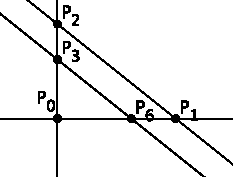
\includegraphics{1_Es6_2a}} 
}
%\hspace{.25in}%
\subfigure[$\alpha^{-1}$]{
\resizebox{6.0 cm}{4.5 cm}{\includegraphics{1_Es6_2b}} 
}
\end{center}%
\caption{Manipolazione di segmenti 2}%
\end{figure}

%%%%%%%%%%%%%%%%%%%%%%%%%%%%%%%%%%%%%%%%%%%%%%%%%%%%%%%%%%%%%% INVERSO
\subsubsection{Inverso del segmento dato}
Si propone, per ultimo, il procedimento per la costruzione di $\alpha^{-1}$.
\begin{enumerate}
\item Dopo aver costruito due rette perpendicolari centrate in $P_{0}$, si pone sull'asse orizzontale il segmento $\alpha$, con estremi $P_{0} P_{1}$.

\item Si tracci il punto $P_{2}$ a distanza $U$ da $P_{0}$, sull'asse orizzontale.

\item Si tracci il punto $P_{3}$ a distanza $U$ da $P_{0}$, sull'asse verticale.

\item Si tracci la retta $R_{4}(P_{1}, P_{3})$, che congiunge gli estremi di $\alpha$ a quelli del segmento unitario verticale.

\item Si tracci la retta $R_{5}$, parallele a $R_{4}$ passante per $P_{2}$, usando il procedimento dell'esempio \ref{parall}.

\item Si evidenzi il punto $P_{6}$ di intersezione fra $R_{5}$ e l'asse verticale.
\end{enumerate}

Nella costruzione appena descritta, vale la seguente proporzione:

\begin{align*}
 \frac{U}{\alpha} = \frac{P_{0}P_{6}}{U}
\end{align*}

dalla quale, ponendo U = 1, si ottiene 

\begin{align*}
P_{0}P_{6} = \alpha^{-1}
\end{align*}

Quindi $P_{0}P_{6}$ è  il segmento di lunghezza $\alpha^{-1}$ cercato. 


%%%%%%%%%%%%%%%%%%% ESEMPIO RADICE
%%
\subsection{Radice quadrata di un segmento dato} \label{radi}

Posto $U = 1$, si vuole costruire un segmento di lunghezza $\sqrt{\alpha}$, dove $\alpha$ è un segmento di lunghezza nota. Si propone la seguente costruzione:

\begin{enumerate}

\item Si tracci il punto $P_{1}$ a distanza $1$ da $P_{0}$ in direzione arbitraria.

\item Si costruiscano i due assi cartesiani ortogonali centrati su $P_0$ con ascisse in direzione $P_1$, utilizzando il procedimento visto in \ref{perp} ed ottenendo quindi la costruzione iniziale
\begin{align*}
S_{1} = ( &P_{0}, P_{1}, R_{2}(P_{0}, P_{1}), C_{3}(P_{0};\overline{P_{0} P_{1}}), \\
&P_{4}(C_{3}, R_{2} ), C_{5}(P_{1};\overline{P_{1} P_{4}}), C_{6}(P_{4};\overline{P_{1} P_{4}}),\\
&P_{7}(C_{5}, C_{6} ), R_{8}(P_{0}, P_{7}) )
\end{align*}
\noindent
Nella figura proposta compariranno per chiarezza solo gli elementi essenziali $P_0, P_1, R_2, P_4, R_8$.

\item Si disegni la circonferenza $C_{9}(P_{0}; \alpha )$  di centro $P_0$ e raggio $\alpha$.

\item Si evidenzi il punto $P_{10}(C_{9}, R_{2} )$, quindi come intersezione fra $C_{3}$ e $R_{2}$. E' stato così ottenuto il segmento $\overline{P_{4}P_{10}}$ di lunghezza $\alpha + 1$.

\item Si trovi il punto medio di $\overline{P_{4} P_{10}}$, dato da $P_{16}$, trovato con il seguente procedimento: 
\begin{align*}
S'_{4} = ( &C_{11}(P_{4}, \overline{P_{4} P_{10}}) ), C_{12}(P_{10}, \overline{P_{10} P_{4}}), \\
&P_{13}(C_{11},C_{12}), P_{14}(C_{11},C_{12}), \\ 
&R_{15}(P_{13}, P_{14}), P_{16}(R_{2},R_{15}) )
\end{align*}
\noindent
analogo a quello usato in \ref{medio}. Nella figura, comparirà per chiarezza solo il punto medio risultante del procedimento e la retta $R_{15}$ passante per esso e perpendicolare a $P_2$.

\item Si tracci la circonferenza $C_{17}(P_{16};\overline{P_{16}P_{10}})$, avente quindi come diametro il segmento $\overline{P_{4}P_{10}}$.

\item Si evidenzi il punto $P_{18}(C_{17}, R_{8} )$.
\end{enumerate}

%%%%%%%% IMMAGINE COSTRUZIONE RADICE QUADRATA %
\begin{figure}[!h]
%centrare
\begin{center}
\resizebox{12.7 cm}{9.5 cm}{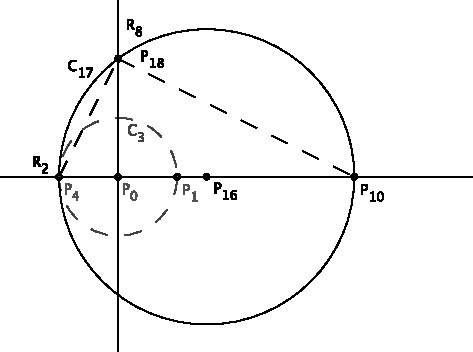
\includegraphics{1_Es7_radice}} 
%\includegraphics{Es1perpendicolare} 
\caption{Radice quadrata di $\alpha$}
\end{center}
\end{figure}

%%%%%%%%%%%%%%%%%%%%%%%%%%%%%%%%%%%%%%% S6

\noindent 
Nella costruzione ottenuta, dato che i triangoli $ P_{4}P_{0} P_{18}$ e $P_{0} P_{18} P_{10}$ sono simili, sussiste la seguente proporzione:
\begin{align*}
P_{4} P_{0} : P_{0} P_{18} = P_{0}P_{18} :P_{0}P_{10}
\end{align*}
Cioè
\begin{align*}
1 : P_{0}P_{18} = P_{0}P_{18} : \alpha
\end{align*}
Da cui si ricava che 
\begin{align*}
P_{0} P_{18} = \sqrt{ \alpha}
\end{align*}
Da questa osservazione si deduce un importante risultato: per ogni segmento dato, di lunghezza $\alpha$, è sempre possibile costruire il segmento di lunghezza $\sqrt{ \alpha}$. 

La costruzione euclidea del procedimento appena descritto è data da:
\begin{align*}
S_{6} = ( &P_{0}, P_{1}, R_{2}(P_{0}, P_{1}), C_{3}(P_{0};\overline{P_{0} P_{1}}), \\
&P_{4}(C_{3}, R_{2} ), C_{5}(P_{1};\overline{P_{1} P_{4}}), C_{6}(P_{4};\overline{P_{1} P_{4}}),\\
&P_{7}(C_{5}, C_{6} ), R_{8}(P_{0}, P_{7}), C_{9}(P_{0}; \alpha ), P_{10}(C_{9}, R_{2} ) \\
&C_{11}(P_{4}, \overline{P_{4} P_{10}}) ), C_{12}(P_{10}, \overline{P_{10} P_{4}}), \\
&P_{13}(C_{11},C_{12}), P_{14}(C_{11},C_{12}),   R_{15}(P_{13}, P_{14}), \\
&P_{16}(R_{2},R_{15}) ), C_{17}(P_{16};\overline{P_{16} P_{10}}), P_{18}(C_{17}, R_{8} ) )
\end{align*}


%FINE CAPITOLO 1
%LABELS

%\label{perp}
%\label{carte}
%\label{bisett}
%\label{medio}
%\label{parall}
%\label{segm}
%\label{radi}

